% questions.tex —— 2004 年·普通高等学校招生考试·湖北卷·文科 · 题目内容片段（无答案）
% 由 tools/generate_projects.py 依来源总账自 2004/2004_数学真题_湖北文科_试题.md 生成，勿手改（改源 MD 后重跑）

\gkpart{一、选择题：本大题共 12 小题，每小题 5 分，共 60 分．在每小题给出的四个选项中，只有一项是符合题目要求的．}

\begin{question}
\gkti{1}设 $A = \{x \mid x = \sqrt{5k + 1}, k \in \mathbf{N}\}$，$B = \{x \mid x \leqslant 6, x \in \mathbf{Q}\}$，则 $A \cap B$ 等于\mbox{（　　）}

\begin{gkopts}(4)
\task A．$\{1, 4\}$
\task B．$\{1, 6\}$
\task C．$\{4, 6\}$
\task D．$\{1, 4, 6\}$
\end{gkopts}

\end{question}
\begin{question}
\gkti{2}已知点 $M_1(6, 2)$ 和 $M_2(1, 7)$．直线 $y = mx - 7$ 与线段 $M_1M_2$ 的交点 $M$ 分有向线段 $M_1M_2$ 的比为 $3 : 2$，则 $m$ 的值为\mbox{（　　）}

\begin{gkopts}(4)
\task A．$-\dfrac{3}{2}$
\task B．$-\dfrac{2}{3}$
\task C．$\dfrac{1}{4}$
\task D．$4$
\end{gkopts}

\end{question}
\begin{question}
\gkti{3}已知函数 $f(x)$ 在 $x = 1$ 处的导数为 $3$，则 $f(x)$ 的解析式可能为\mbox{（　　）}

\begin{gkopts}(2)
\task A．$f(x) = (x - 1)^2 + 3(x - 1)$
\task B．$f(x) = 2(x - 1)$
\task C．$f(x) = 2(x - 1)^2$
\task D．$f(x) = x - 1$
\end{gkopts}

\end{question}
\begin{question}
\gkti{4}两个圆 $C_1: x^2 + y^2 + 2x + 2y - 2 = 0$ 与 $C_2: x^2 + y^2 - 4x - 2y + 1 = 0$ 的公切线有且仅有\mbox{（　　）}

\begin{gkopts}(4)
\task A．$1$ 条
\task B．$2$ 条
\task C．$3$ 条
\task D．$4$ 条
\end{gkopts}

\end{question}
\begin{question}
\gkti{5}若函数 $f(x) = a^x + b - 1$（$a > 0, a \neq 1$）的图象经过第二、三、四象限，则一定有\mbox{（　　）}

\begin{gkopts}(2)
\task A．$0 < a < 1$，且 $b > 0$
\task B．$a > 1$，且 $b > 0$
\task C．$0 < a < 1$，且 $b < 0$
\task D．$a > 1$，且 $b < 0$
\end{gkopts}

\end{question}
\begin{question}
\gkti{6}四面体 $ABCD$ 四个面的重心分别为 $E$、$F$、$G$、$H$，则四面体 $EFGH$ 的表面积与四面体 $ABCD$ 的表面积的比值是\mbox{（　　）}

\begin{gkopts}(4)
\task A．$\dfrac{1}{27}$
\task B．$\dfrac{1}{16}$
\task C．$\dfrac{1}{9}$
\task D．$\dfrac{1}{8}$
\end{gkopts}

\end{question}
\begin{question}
\gkti{7}已知 $\vec{a}, \vec{b}, \vec{c}$ 为非零的平面向量．甲：$\vec{a} \cdot \vec{b} = \vec{a} \cdot \vec{c}$，乙：$\vec{b} = \vec{c}$，则\mbox{（　　）}

\begin{gkopts}(2)
\task A．甲是乙的充分条件但不是必要条件
\task B．甲是乙的必要条件但不是充分条件
\task C．甲是乙的充要条件
\task D．甲既不是乙的充分条件也不是乙的必要条件
\end{gkopts}

\end{question}
\begin{question}
\gkti{8}已知 $x \geqslant \dfrac{5}{2}$，则 $f(x) = \dfrac{x^2 - 4x + 5}{2x - 4}$ 有\mbox{（　　）}

\begin{gkopts}(2)
\task A．最大值 $\dfrac{5}{4}$
\task B．最小值 $\dfrac{5}{4}$
\task C．最大值 $1$
\task D．最小值 $1$
\end{gkopts}

\end{question}
\begin{question}
\gkti{9}设数列 $\{a_n\}$ 的前 $n$ 项和 $S_n = a\left[2 - \left(\dfrac{1}{2}\right)^{n-1}\right] - b\left[2 - (n + 1)\left(\dfrac{1}{2}\right)^{n-1}\right]$（$n = 1, 2, \cdots$），其中 $a$、$b$ 是非零常数．则存在数列 $\{x_n\}$、$\{y_n\}$ 使得\mbox{（　　）}

\begin{gkopts}(1)
\task A．$a_n = x_n + y_n$，其中 $\{x_n\}$ 为等差数列，$\{y_n\}$ 为等比数列
\task B．$a_n = x_n + y_n$，其中 $\{x_n\}$ 和 $\{y_n\}$ 都为等差数列
\task C．$a_n = x_n \cdot y_n$，其中 $\{x_n\}$ 为等差数列，$\{y_n\}$ 为等比数列
\task D．$a_n = x_n \cdot y_n$，其中 $\{x_n\}$ 和 $\{y_n\}$ 都为等比数列
\end{gkopts}

\end{question}
\begin{question}
\gkti{10}若 $1 < \dfrac{1}{a} < \dfrac{1}{b}$，则下列结论中不正确的是\mbox{（　　）}

\begin{gkopts}(1)
\task A．$\log_a b > \log_b a$
\task B．$|\log_a b + \log_b a| > 2$
\task C．$(\log_b a)^2 < 1$
\task D．$|\log_a b| + |\log_b a| > |\log_a b + \log_b a|$
\end{gkopts}

\end{question}
\begin{question}
\gkti{11}将标号为 $1, 2, \cdots, 10$ 的 $10$ 个球放入标号为 $1, 2, \cdots, 10$ 的 $10$ 个盒子里，每个盒内放一个球，恰好 $3$ 个球的标号与其在盒子的标号不一致的放入方法种数为\mbox{（　　）}

\begin{gkopts}(4)
\task A．$120$
\task B．$240$
\task C．$360$
\task D．$720$
\end{gkopts}

\end{question}
\begin{question}
\gkti{12}设 $y = f(t)$ 是某港口水的深度 $y$（米）关于时间 $t$（时）的函数，其中 $0 \leqslant t \leqslant 24$，下表是该港口某一天从 $0$ 时至 $24$ 时记录的时间 $t$ 与水深 $y$ 的关系：

\begin{center}
\begingroup\setlength{\tabcolsep}{4pt}
\begin{tabular}{cccccccccc}
\toprule
$t$ & $0$ & $3$ & $6$ & $9$ & $12$ & $15$ & $18$ & $21$ & $24$ \\
\midrule
$y$ & $12$ & $15.1$ & $12.1$ & $9.1$ & $11.9$ & $14.9$ & $11.9$ & $8.9$ & $12.1$ \\
\bottomrule
\end{tabular}
\endgroup
\end{center}

经长期观察，函数 $y = f(t)$ 的图象可以近似地看成函数 $y = k + A\sin(\omega t + \varphi)$ 的图象．下面的函数中，最能近似表示表中数据间对应关系的函数是\mbox{（　　）}

\begin{gkopts}(1)
\task A．$y = 12 + 3\sin\dfrac{\pi}{6}t, t \in [0, 24]$
\task B．$y = 12 + 3\sin\left(\dfrac{\pi}{6}t + \pi\right), t \in [0, 24]$
\task C．$y = 12 + 3\sin\dfrac{\pi}{12}t, t \in [0, 24]$
\task D．$y = 12 + 3\sin\left(\dfrac{\pi}{12}t + \dfrac{\pi}{2}\right), t \in [0, 24]$
\end{gkopts}

\end{question}
\gkpart{二、填空题：本大题共 4 小题，每小题 4 分，共 16 分．把答案填在题中横线上．}

\begin{question}
\gkti{13}$\tan 2010^\circ$ 的值为 $\underline{\quad\quad}$．

\end{question}
\begin{question}
\gkti{14}已知 $\left(x^{\frac{1}{2}} + x^{-\frac{1}{2}}\right)^n$ 的展开式中各项系数的和是 $128$，则展开式中 $x^5$ 的系数是 $\underline{\quad\quad}$．（以数字作答）

\end{question}
\begin{question}
\gkti{15}某校有老师 $200$ 人，男学生 $1200$ 人，女学生 $1000$ 人．现用分层抽样的方法从所有师生中抽取一个容量为 $n$ 的样本；已知从女学生中抽取的人数为 $80$ 人，则 $n = \underline{\quad\quad}$．

\end{question}
\begin{question}
\gkti{16}设 $A$、$B$ 为两个集合．下列四个命题：

① $A \not\subseteq B \iff$ 对任意 $x \in A$，有 $x \notin B$；

② $A \not\subseteq B \iff A \cap B = \varnothing$；

③ $A \not\subseteq B \iff A \not\supseteq B$；

④ $A \not\subseteq B \iff$ 存在 $x \in A$，使得 $x \notin B$．

其中真命题的序号是 $\underline{\quad\quad}$．（把符合要求的命题序号都填上）

\end{question}
\gkpart{三、解答题：本大题共 6 小题，共 74 分．解答应写出文字说明、证明过程或演算步骤．}

\begin{question}
\gkti{17}已知 $6\sin^2\alpha + \sin\alpha\cos\alpha - 2\cos^2\alpha = 0$，$\alpha \in \left[\dfrac{\pi}{2}, \pi\right]$，求 $\sin\left(2\alpha + \dfrac{\pi}{3}\right)$ 的值．

\Needspace{0.4\textheight}
\end{question}
\begin{question}
\gkti{18}如图，在棱长为 $1$ 的正方体 $ABCD - A_1B_1C_1D_1$ 中，$AC$ 与 $BD$ 交于点 $E$，$C_1B$ 与 $CB_1$ 交于点 $F$．

（1）求证：$A_1C \perp$ 平面 $BDC_1$；

（2）求二面角 $B - EF - C$ 的大小．（结果用反三角函数值表示）
\nopagebreak[4]
\begin{center}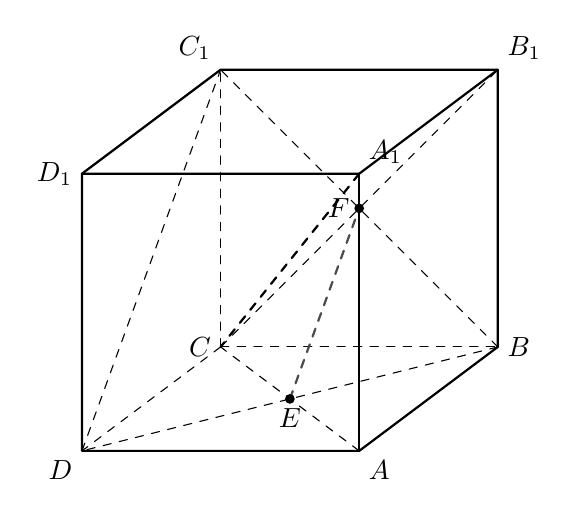
\begin{tikzpicture}[scale=2.2, line join=round, line cap=round, >=stealth]
  % 顶点坐标设定（斜二测投影）
  \coordinate (C) at (0, 0);
  \coordinate (D) at (-0.8, -0.6);
  \coordinate (A) at (0.8, -0.6);
  \coordinate (B) at (1.6, 0);

  \coordinate (C1) at (0, 1.6);
  \coordinate (D1) at (-0.8, 1.0);
  \coordinate (A1) at (0.8, 1.0);
  \coordinate (B1) at (1.6, 1.6);

  % 交点坐标
  \coordinate (E) at (0.4, -0.3); % AC 与 BD 交点
  \coordinate (F) at (0.8, 0.8);  % C1B 与 CB1 交点

  % 虚线部分（内部与后侧）
  \draw[dashed, thin] (C) -- (D);
  \draw[dashed, thin] (C) -- (B);
  \draw[dashed, thin] (C) -- (C1);
  \draw[dashed, thin] (A) -- (C);
  \draw[dashed, thin] (B) -- (D);
  \draw[dashed, thin] (C) -- (B1);
  \draw[dashed, thin] (B) -- (C1);
  \draw[dashed, thick] (A1) -- (C);
  \draw[dashed, thin] (D) -- (C1);
  \draw[dashed, thick, black!70] (E) -- (F);

  % 实线部分（外轮廓与前侧）
  \draw[thick] (D) -- (A) -- (B) -- (B1) -- (C1) -- (D1) -- cycle;
  \draw[thick] (A) -- (A1);
  \draw[thick] (D1) -- (A1) -- (B1);

  % 顶点标注
  \node[left] at (C) {$C$};
  \node[below left] at (D) {$D$};
  \node[below right] at (A) {$A$};
  \node[right] at (B) {$B$};
  \node[above left] at (C1) {$C_1$};
  \node[left] at (D1) {$D_1$};
  \node[above right] at (A1) {$A_1$};
  \node[above right] at (B1) {$B_1$};
  \node[below] at (E) {$E$};
  \node[left] at (F) {$F$};

  % 关键点标记
  \fill (E) circle (0.8pt);
  \fill (F) circle (0.8pt);
\end{tikzpicture}
\end{center}
\nopagebreak[4]
\Needspace{0.4\textheight}
\end{question}
\begin{question}
\gkti{19}如图，在 $\mathrm{Rt}\triangle ABC$ 中，已知 $BC = a$，若长为 $2a$ 的线段 $PQ$ 以点 $A$ 为中点，问 $\vec{PQ}$ 与 $\vec{BC}$ 的夹角 $\theta$ 取何值时 $\vec{BP} \cdot \vec{CQ}$ 的值最大？并求出这个最大值．
\nopagebreak[4]
\begin{center}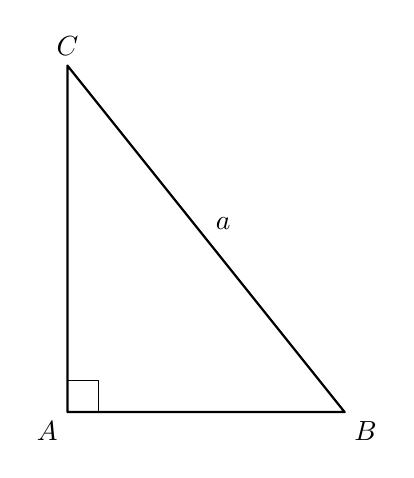
\begin{tikzpicture}[scale=2.2, line join=round, line cap=round]
  \coordinate (A) at (0, 0);
  \coordinate (B) at (1.6, 0);
  \coordinate (C) at (0, 2.0);

  % 绘制直角三角形
  \draw[thick] (A) -- (B) -- (C) -- cycle;

  % 直角标记
  \draw[thin] (0, 0.18) -- (0.18, 0.18) -- (0.18, 0);

  % 顶点与边长标注
  \node[below left] at (A) {$A$};
  \node[below right] at (B) {$B$};
  \node[above] at (C) {$C$};
  \node[above right] at (0.8, 1.0) {$a$};
\end{tikzpicture}
\end{center}
\nopagebreak[4]
\end{question}
\begin{question}
\gkti{20}直线 $l: y = kx + 1$ 与双曲线 $C: 2x^2 - y^2 = 1$ 的右支交于不同的两点 $A$、$B$．

（1）求实数 $k$ 的取值范围；

（2）是否存在实数 $k$，使得以线段 $AB$ 为直径的圆经过双曲线 $C$ 的右焦点 $F$？若存在，求出 $k$ 的值．若不存在，说明理由．

\end{question}
\begin{question}
\gkti{21}为防止某突发事件发生，有甲、乙、丙、丁四种相互独立的预防措施可供采用，单独采用甲、乙、丙、丁预防措施后此突发事件不发生的概率（记为 $P$）和所需费用如下表：

\begin{center}
\begin{tabular}{lcccc}
\toprule
预防措施 & 甲 & 乙 & 丙 & 丁 \\
\midrule
$P$ & $0.9$ & $0.8$ & $0.7$ & $0.6$ \\
费用（万元） & $90$ & $60$ & $30$ & $10$ \\
\bottomrule
\end{tabular}
\end{center}

预防方案可单独采用一种预防措施或联合采用几种预防措施，在总费用不超过 $120$ 万元的前提下，请确定一个预防方案，使得此突发事件不发生的概率最大．

\end{question}
\begin{question}
\gkti{22}已知 $b > -1$，$c > 0$，函数 $f(x) = x + b$ 的图象与函数 $g(x) = x^2 + bx + c$ 的图象相切．

（1）求 $b$ 与 $c$ 的关系式（用 $c$ 表示 $b$）；

（2）设函数 $F(x) = f(x)g(x)$ 在 $(-\infty, +\infty)$ 内有极值点，求 $c$ 的取值范围．

\end{question}